%
% teil3.tex -- Beispiel-File für Teil 3
%
% (c) 2020 Prof Dr Andreas Müller, Hochschule Rapperswil
%
% !TEX root = ../../buch.tex
% !TEX encoding = UTF-8
%
\section{Luftwiderstand\label{ueberschall:section:Luftwiderstand}}
\kopfrechts{Luftwiderstand}
Wenige physikalisches Phänomene begegnen uns so oft und bleiben
so unsichtbar wie der Luftwiderstand.
Ebenso ist die Berechnung des Luftwiderstandes eines Objektes die beliebteste
Anwendung der Gleichungen, die wir im vorherigen Kapitel behandelt haben.
Insbesondere das Objekt mit dem minimalen Widerstand der Sears-Haack Körper.

\subsection{Theoretischer und realer Luftwiderstand}
Wenn wir mithilfe der Strömungsgleichungen den Druck genauer analysieren,
können wir den Verlauf des Luftwiderstands zeigen, 
wie in Abbildung~\ref{fig:luftwiderstand}.
\begin{figure}
    \centering
    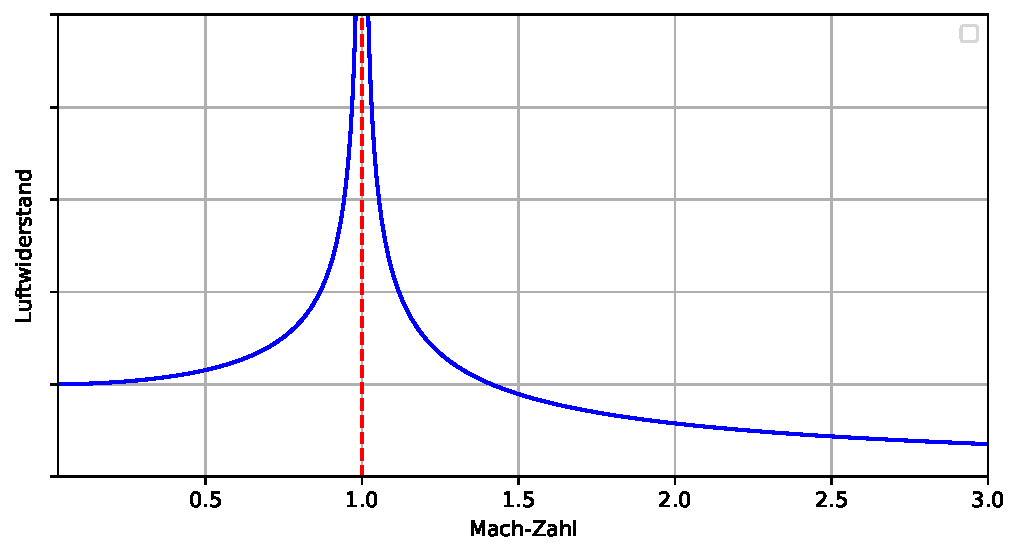
\includegraphics[width=\textwidth]{papers/ueberschall/figures/Luftwiderstand_qual.pdf}
    \caption{Qualitativer Verlauf des Luftwiderstands.}
    ~\label{fig:luftwiderstand}
\end{figure}
Man stellt schnell fest, dass diese Betrachtung nicht der Realität
entspricht.
Gemäss diesen Formeln müsste man eine unendliche Kraft überwinden,
um die Schallgeschwindigkeit zu erreichen, 
welche heutzutage schon zivile Flugzeuge ohne weiteres überschreiten.
Das erklärt auch warum in Abbildung~\ref{fig:abklingen_stromlinie}
für Geschwindigkeiten sehr nahe der Schallgeschwindigkeit, die Krümmung in 
den Stromlinien kaum abklingt.
Deswegen wird an dieser Stelle erneut daran erinnert, dass es sich bei den Lösungen
um vereinfachte Approximationen handelt, da für die exakte Differentialgleichung
bisher keine strenge Lösung gefunden werden konnte.
(Gleichung 5 aus Paper evtl. postulieren)
Nichtsdestotrotz ist anzumerken, dass das Verhalten
um die Schallgeschwindigkeit herum qualitativ korrekt ist.
Die Strömungskräfte nehmen im Unterschall zu und im Überschall
nehmen sie langsam wieder ab.

Um das nun zu vergleichen brauchen wir ein reales Beispiel mit
empirisch ermittelten Werten.
Dafür nehmen wir ein 50 Kaliber M33 Projektil.
Wir sehen in Abbildung~\ref{fig:luftwiderstand_50-M33}
im Übergangsbereich von Unterschall zu Überschall
, wie der Luftwiderstand stark ansteigt
und nach dem Überschreiten der Schallgeschwindigkeit bei ca. $1.2\,\mathrm{Mach}$
dieser wieder sinkt.
Das Maximum bzw. der Buckel im transsonischen Bereich bleibt bis heute unerklärt.
\begin{figure}
    \centering
    \begin{minipage}[t]{0.4\textwidth}
        \centering
        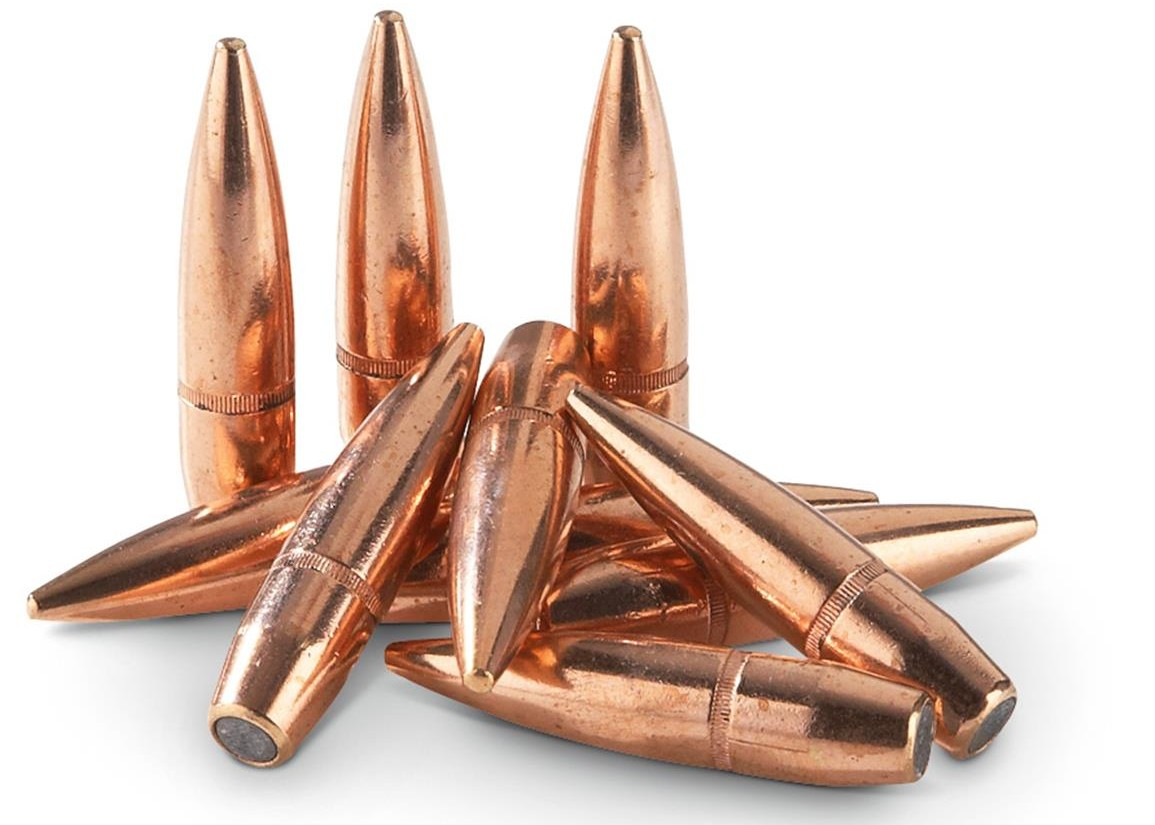
\includegraphics[width=\linewidth]{papers/ueberschall/figures/50-cal_projectile.jpg}
        \caption*{50 Kaliber M33 Projektil~\cite{ArmoryFarm50BMG}.}
    \end{minipage}
    \hfill
    \begin{minipage}[t]{0.55\textwidth}
        \centering
        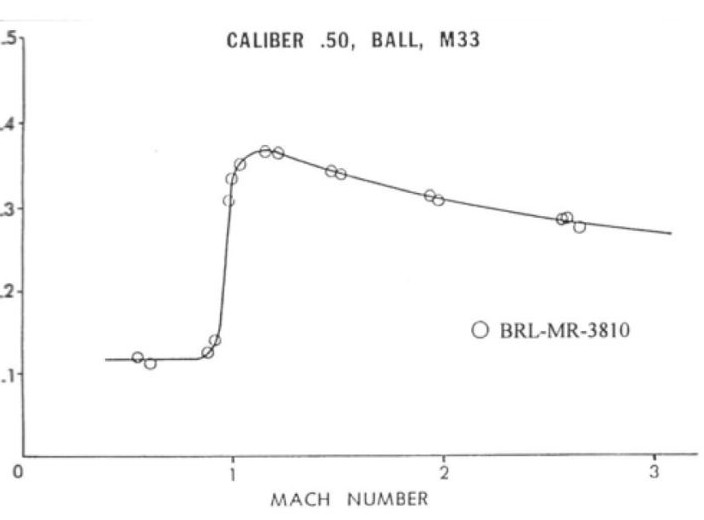
\includegraphics[width=\linewidth]{papers/ueberschall/figures/50-M33 Geschoss.jpg}
        \caption*{Luftwiderstand als Funktion der Machzahl~\cite{Mittelkaliber2020}.}
    \end{minipage}
    \caption{Projektil und Luftwiderstandskurve für ein 50-M33 Geschoss.}
    ~\label{fig:luftwiderstand_50-M33}
\end{figure}

\subsection{Physikalische bedeutung des widerstands}
im unterschall ist es der Druck.
im Überschall ist es der Wellenwiderstand-> shock wave (machkegeln)